\def\stitle{\theexercise\ - Anweisungen 1}
\section{\stitle}
\begin{frame}[t]%
    \frametitle{\stitle}

Gegeben sei der folgende Ausschnitt eines Java-Programms. Sei \code{n} vom Typ \code{int}.

\lstinputlisting[style=JAVAsmalllines]{anweis-1/Anweis1_snippet.java}

\begin{itemize}
\item[a)] Welcher Buchstabe wird auf dem Bildschirm ausgegeben, falls \code{n} den Wert $1$, $2$, $3$ bzw. $4$ besitzt?
\end{itemize}
\end{frame}


%%%%%%%%%%%%%%%%%%%%%%%%%%%%%%%%%%%%%%%%%%%%%%%%%%%%%%%%%%%%%%%%%%%%%%%%
\begin{frame}[fragile]%
 \frametitle{a) Struktogramm mit Java-Editor}%

\begin{center}
\lstinputlisting[style=JAVAlines]{anweis-1/Anweis1_snippet.java}
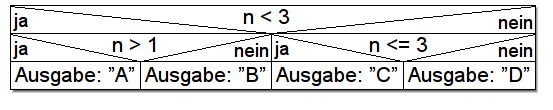
\includegraphics[width=0.8\textwidth]{anweis-1/Bilder/Struktogramm_a}
\end{center}

\end{frame}

\begin{frame}[t]%
    \frametitle{\stitle}

Gegeben sei der folgende Ausschnitt eines Java-Programms. Sei \code{n} vom Typ \code{int}.

\lstinputlisting[style=JAVAsmalllines]{anweis-1/Anweis1_snippet.java}

\begin{itemize}
\item[b)] Welcher Buchstabe wird auf dem Bildschirm ausgegeben, falls \code{n} den Wert $1$, $2$, $3$ bzw. $4$ besitzt und \textbf{jeder} Boolsche Ausdruck in dem Programmabschnitt durch seine Negation ersetzt wurde?
\end{itemize}
\end{frame}

%%%%%%%%%%%%%%%%%%%%%%%%%%%%%%%%%%%%%%%%%%%%%%%%%%%%%%%%%%%%%%%%%%%%%%%%
\begin{frame}[fragile]%
\frametitle{b) Strukturprogramm mit Java-Editor}%
\begin{center}
\lstinputlisting[style=JAVAlines]{anweis-1/Anweis1_snippet.java}
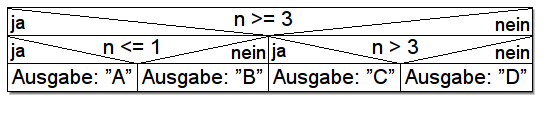
\includegraphics[width=0.8\textwidth]{anweis-1/Bilder/Struktogramm_b}
\end{center}

\end{frame}


%%%%%%%%%%%%%%%%%%%%%%%%%%%%%%%%%%%%%%%%%%%%%%%%%%%%%%%%%%%%%%%%%%%%%%%%
\begin{frame}[fragile]%
 \frametitle{c) Beispiel Programm}%
\lstinputlisting[style=JAVAsmall,title={Programm zur Aufgabe Anweisungen.}]{anweis-1/Anweis1.java}
\end{frame}
